\documentclass{scrartcl}  % Was möchte ich schreiben scrartcl--> Artikel

\usepackage[utf8x]{inputenc}  % Umlaute etc. im Input-File
\usepackage[T1]{fontenc}	% Datestellung der Umlaute im Ouput-File
\usepackage{lmodern}	% für bessere Darstellung im Pdf
\usepackage{amsmath, amssymb, amstext, amsthm}
\usepackage{hyperref}	%aktiviert Hyperrefs
\usepackage{threeparttable}
\usepackage{graphicx}
\usepackage{wrapfig}
\usepackage{array}
\usepackage{float}
\usepackage{underscore}
\usepackage{listings}

\lstset{language=Python}
\lstset{basicstyle=\footnotesize}
\setlength{\parindent}{0em}


\usepackage[naustrian]{babel}	% Rechtschreibung für Österreichisch aktivieren

\title{YoMoPi - Library}
\author{Stefan Jost}

\usepackage[automark]{scrpage2}	% Kopf und Fußzeile hinzufügen
\pagestyle{scrheadings}
\clearscrheadfoot
\ifoot[\pagemark]{\pagemark}
\ofoot[YoMoPi - Library]{YoMoPi - Library}
\chead[YoMoPi - Library]{YoMoPi - Library}



\begin{document}

\maketitle  % Titel erzeugen mit den oben angeführten Parametern
\newpage
\tableofcontents
\newpage

\section{Imports}
Following imports were needed for this library.

\textbf{time}: time was needed to get the timestamp on each value.

\textbf{math}: math was needed to calculate the squareroot for the reactive energy.

\textbf{spidev}: the spidev module was needed to use the SPI on the Raspberry Pi

\textbf{sys}: 

\textbf{RPi.GPIO}: the RPi.GPIO was needed to controll the GPIO pins for the reset pin and further extentions

\begin{lstlisting}
import time
import math
import spidev
import sys
import RPi.GPIO as GPIO 
\end{lstlisting}
 
\section{Classvariables}

Following variable were needed to correcty access the register and to adjust the register values to usefull values. 

\textbf{read} and \textbf{write}: the read and write were needed to mask the register address to not accidently write the register instead of reading it. Therefor to read a register the given address will be bitwise AND masked with the \textbf{read} variable and to write a register the address will be bitwise OR masked with the \textbf{write} variable.

\textbf{spi}, \textbf{active_lines} and \textbf{debug}: this variables were used to save the spi object, to save the number of actives phases that will be measured and to enable debugging via the console.

\textbf{sampleintervall}, \textbf{active_factor}, \textbf{apparent_factor}, \textbf{vrms_factor} and \textbf{irms_factor}: the sampleintervall defines the time between each sample when the start_sampling method is called. The minimum time between each sample is 1 second. Sampleintervall defines the number of seconds and can take each integer value greater then 0. The different factor variables will adjust the values read from the registers. This factors can be changes but should not be changed because they are calibrated values.
\begin{lstlisting}
read = 0b00111111
write = 0b10000000
spi=0
active_lines = 1
debug = 1
	
sampleintervall = 1
active_factor = 1
apparent_factor = 1
vrms_factor = 1
irms_factor = 1
\end{lstlisting}
    
\section{Methods}

In this section every method from the library is listed and you will find a detailed description on the parameters and returns of each function. For more information you will also find the full source code of the function.
\subsection{__init__}


\textbf{Description}: This is the constructor and it creates a new YoMoPi object. It also creates a new SPI objects for each YoMoPi object.

\textbf{Parameters}: None.

\textbf{Returns}: Nothing.
\begin{lstlisting}
def __init__(self):
       self.spi=spidev.SpiDev()
       return 
\end{lstlisting}
 
\subsection{init_yomopi}

\textbf{Description}: Initializes the YoMoPi object. Sets the GPIO mode, disables GPIO warnings and defines pin 19 as output. Also opens a new SPI connection via the SPI device (0,0), sets the SPI speed to 62500 Hz and sets the SPI mode to 1. Finaly the function set_lines is called to set the MMODE, WATMODE and VAMODE.

\textbf{Parameters}: None.

\textbf{Returns}: Nothing.

\begin{lstlisting}
def init_yomopi(self):
	GPIO.setmode(GPIO.BCM)
       GPIO.setwarnings(False)
       GPIO.setup(19,GPIO.OUT)
       self.spi.open(0,0)
       self.spi.max_speed_hz = 62500
       self.spi.mode = 0b01
	self.set_lines(self.active_lines)
       return 
\end{lstlisting}
		
\subsection{set_lines}

\textbf{Description}: This function sets the number of active phases that will be measured.

\textbf{Parameters}: lines - 1 or 3

\textbf{Returns}: Nothing.
\begin{lstlisting}
def set_lines(self, lines):
	if (lines != 1) and (lines != 3):
       	print "Wrong number of lines"
            	return
	else:
           	self.active_lines = lines
            	if self.active_lines == 3:
			self.write_8bit(0x0D, 0x3F)
                	self.write_8bit(0x0E, 0x3F)
			self.set_mmode(0x70)
            	elif self.active_lines == 1:
            		self.write_8bit(0x0D, 0x24)
            		self.write_8bit(0x0E, 0x24)	
            		self.set_mmode(0x10)				
		return
	return
\end{lstlisting}

\subsection{enable_board}

\textbf{Description}: Enables the board by pulling pin 19 into the HIGH state.

\textbf{Parameters}: None.

\textbf{Returns}: Nothing.

\begin{lstlisting}	
def enable_board(self):
	GPIO.output(19, GPIO.HIGH)
	return
\end{lstlisting}

\subsection{disable_board}

\textbf{Description}: Disables the board by pulling pin 19 into the LOW state.

\textbf{Parameters}: None.

\textbf{Returns}: Nothing.

\begin{lstlisting}
def disable_board(self):
       GPIO.output(19, GPIO.LOW)
       return
\end{lstlisting}

\subsection{write_8bit}    

\textbf{Description}: Writes 8 bit of data to the given address.

\textbf{Parameters}: register - 8 bit address of the register (see ADE7754 register table)

					value - 8 bit of value that will be written into the register

\textbf{Returns}: Nothing.

\begin{lstlisting}
def write_8bit(self, register, value):
       self.enable_board()
       register = register | self.write
       self.spi.xfer2([register, value])
       return
\end{lstlisting}

\subsection{read_8bit}

\textbf{Description}: Reads 8 bit of data from the given address.

\textbf{Parameters}: register - 8 bit address of the register (see ADE7754 register table)

\textbf{Returns}: the 8 bit of data in the register as decimal

\begin{lstlisting}
def read_8bit(self, register):
       self.enable_board()
       register = register \& self.read
       result = self.spi.xfer2([register, 0x00])[1:]        
       return result[0]
\end{lstlisting}
 
\subsection{read_16bit}   

\textbf{Description}: Reads 16 bit of data from the given address.

\textbf{Parameters}: register - 8 bit address of the register (see ADE7754 register table)

\textbf{Returns}: the 16 bit of data in the register as decimal
  
\begin{lstlisting}
def read_16bit(self, register):
       self.enable_board()
       register = register \& self.read
       result = self.spi.xfer2([register, 0x00, 0x00])[1:]
       dec_result = (result[0]<<8)+result[1]
       return dec_result
\end{lstlisting}

\subsection{read_24bit}        

\textbf{Description}: Reads 24 bit of data from the given address.

\textbf{Parameters}: register - 8 bit address of the register (see ADE7754 register table)

\textbf{Returns}: the 24 bit of data in the register as decimal

\begin{lstlisting}
def read_24bit(self, register):
       self.enable_board()
       register = register \& self.read
       result = self.spi.xfer2([register, 0x00, 0x00, 0x00])[1:]
       dec_result = (result[0]<<16)+(result[1]<<8)+(result[0])
       return dec_result
\end{lstlisting}

\subsection{get_temp}

\textbf{Description}: Reads 8 bit of data from the temperature register (0x08).

\textbf{Parameters}: None.

\textbf{Returns}: A list of two elements [timestamp, temperature in °C]

\begin{lstlisting}
def get_temp(self):
       reg = self.read_8bit(0x08)
       temp = [time.time(),(reg-129)/4]
       return temp
\end{lstlisting}
    
\subsection{get_aenergy}

\textbf{Description}: Reads 24 bit of data from the active ernergy register (0x02) and resets the register to 0.

\textbf{Parameters}: None.

\textbf{Returns}: A list of two elements [timestamp, value of the register]

\begin{lstlisting}
def get_aenergy(self):
       aenergy = [time.time(), self.read_24bit(0x02)]
       return aenergy
\end{lstlisting}

\subsection{get_appenergy}	

\textbf{Description}: Reads 24 bit of data from the apparent ernergy register (0x05) and resets the register to 0.

\textbf{Parameters}: None.

\textbf{Returns}: A list of two elements [timestamp, value of the register]
\begin{lstlisting}	
def get_appenergy(self):
	appenergy = [time.time(), self.read_24bit(0x05)]
    	return appenergy
\end{lstlisting}
 
\subsection{get_period}   

\textbf{Description}: Reads 16 bit of data from the period register (0x07).

\textbf{Parameters}: None.

\textbf{Returns}: A list of two elements [timestamp, value of the register]
\begin{lstlisting}
def get_period(self):
       period = [time.time(), self.read_16bit(0x07)]
       return period
\end{lstlisting}
		
\subsection{set_opmode}

\textbf{Description}: Sets the OPMODE. For more information to the OPMODE see section OPMODE.

\textbf{Parameters}: value - 8 bit of data representing the OPMODE

\textbf{Returns}: Nothing.

\begin{lstlisting}
def set_opmode(self, value):
	self.write_8bit(0x0A, value)
    	return
\end{lstlisting}

\subsection{set_mmode}

\textbf{Description}: Sets the MMODE. For more information to the MMODE see section MMODE.

\textbf{Parameters}: value - 8 bit of data representing the MMODE

\textbf{Returns}: Nothing.

\begin{lstlisting}
def set_mmode(self, value):
	self.write_8bit(0x0B, value)
    	return
\end{lstlisting}

\subsection{get_sample}	

\textbf{Description}: Takes one sample and calculates the active energy, apparent energy, reactive energy, VRMS and IRMS. The calculated values are the real values. (after adjusting with their factores)

\textbf{Parameters}: None.

\textbf{Returns}: A list of 7 elements [timestamp, active energy, apparent energy, reactive energy, period, VRMS, IRMS]

\begin{lstlisting}	
def get_sample(self):
    	aenergy = self.get_aenergy()[1] *self.active_factor
    	appenergy = self.get_appenergy()[1] *self.apparent_factor 
    	renergy = math.sqrt(appenergy*appenergy - aenergy*aenergy)
    	if self.debug:
    		print"Active energy: %f W, Apparent energy: %f VA, Reactive Energy: %f var" 
		% (aenergy, appenergy, renergy)
    		print"VRMS: %f IRMS: %f" 
		%(self.get_vrms()[1]*self.vrms_factor,self.get_irms()[1]*self.irms_factor)
    	sample = []
    	sample.append(time.time())
    	sample.append(aenergy)
    	sample.append(appenergy)
    	sample.append(renergy)
    	sample.append(self.get_period()[1])
    	sample.append(self.get_vrms()[1]*self.vrms_factor)
    	sample.append(self.get_irms()[1]*self.irms_factor)
    	return sample
\end{lstlisting}
		
\subsection{get_vrms}

\textbf{Description}: Reads the VRMS register depending on if the active lines is 1 or 3.

\textbf{Parameters}: None.

\textbf{Returns}: A list of 2 elements [timestamp, Phase A VRMS] or 4 elements [timestamp, Phase A VRMS, Phase B VRMS, Phase C VRMS]

\begin{lstlisting}
def get_vrms(self):
    	if self.active_lines == 1:
    		avrms = [time.time(), self.read_24bit(0x2C)]
    		return avrms
    	elif self.active_lines == 3:
              vrms = []
              vrms.append(time.time())
    		vrms.append(self.read_24bit(0x2C))
    		vrms.append(self.read_24bit(0x2D))
    		vrms.append(self.read_24bit(0x2E))
    		return vrms
	return 0
\end{lstlisting}
		
\subsection{get_irms}

\textbf{Description}: Reads the IRMS register depending on if the active lines is 1 or 3.

\textbf{Parameters}: None.

\textbf{Returns}: A list of 2 elements [timestamp, Phase A IRMS] or 4 elements [timestamp, Phase A IRMS, Phase B IRMS, Phase C IRMS]

\begin{lstlisting}
def get_irms(self):
    	if self.active_lines == 1:
    		airms = [time.time(), self.read_24bit(0x29)]
    		return airms
    	elif self.active_lines == 3:
              irms = []
              irms.append(time.time())
    		irms.append(self.read_24bit(0x29))
    		irms.append(self.read_24bit(0x2A))
    		irms.append(self.read_24bit(0x2B))
    		return vrms
    	return 0
\end{lstlisting}
		
\subsection{start_sampling}	

\textbf{Description}: Starts a sampling programm that takes a number of samples depending on the parameters.

\textbf{Parameters}: nr_samples - this are the number of samples that will be taken, integer greater then 0

					samplerate - this is the time between each sample, integer greater then 0

\textbf{Returns}: A list of samples (each sample is a list of 7 elements)
\begin{lstlisting}
def start_sampling(self, nr_samples, samplerate):
	if (samplerate<1) or (nr_samples<1):
		return 0
	self.sampleintervall = samplerate
	samples = []
	for i in range(0, nr_samples):
            
		for j in range(0, samplerate):
			time.sleep(1)
                
		samples.append(self.get_sample())     
	return samples
\end{lstlisting}
    
\subsection{close}

\textbf{Description}: Closes the SPI connection.

\textbf{Parameters}: None.

\textbf{Returns}: Nothing.

\begin{lstlisting}
def close(self):
	self.spi.close()
	return
\end{lstlisting}

\section{OPMODE}
The general configuration of the ADE7754 is defined by writing to the OPMODE register (0x0A).
\begin{figure}[H]
\centering
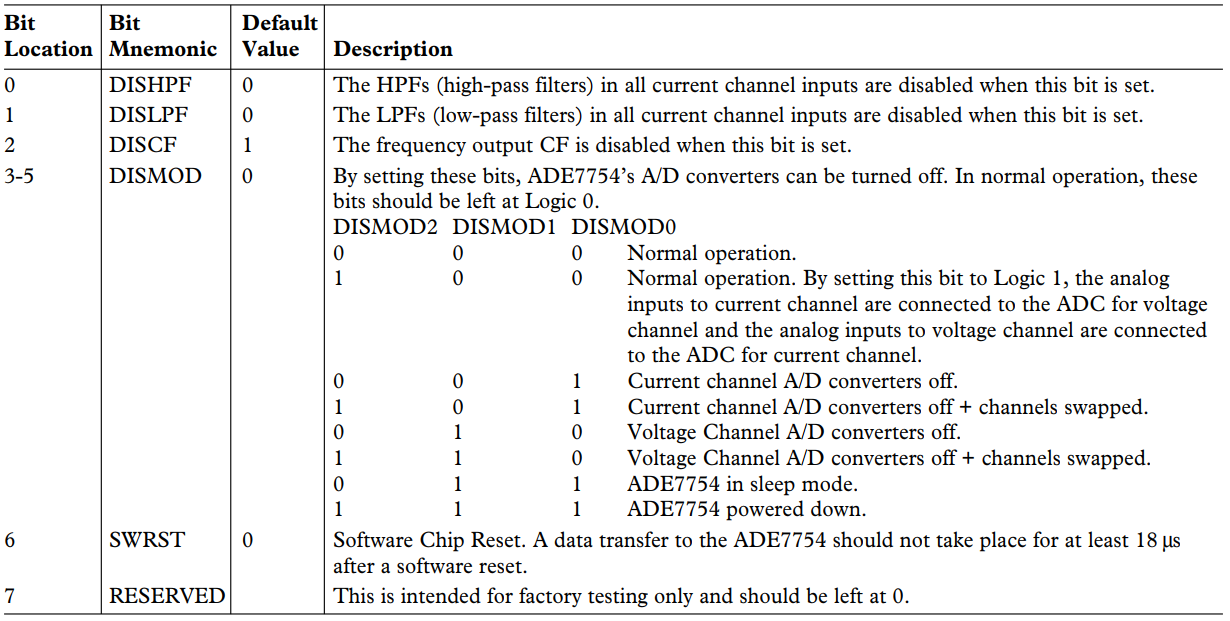
\includegraphics[width=1\textwidth]{opmode.png}
\caption{OPMODE}\label{fig:myFigure1}
\end{figure}

\newpage

\section{MMODE}
The configuration of the period and peak measurements made by the ADE7754 are defined by writing to the MMODE register (0x0B).
\begin{figure}[H]
\centering
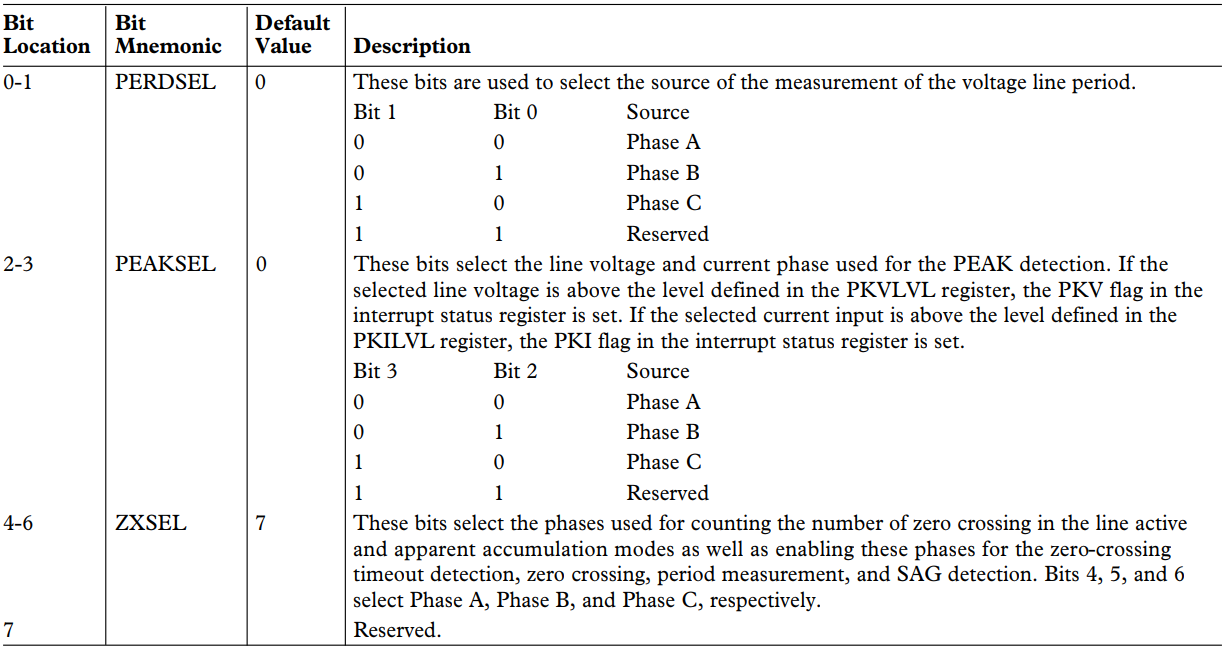
\includegraphics[width=1\textwidth]{mmode.png}
\caption{MMODE}\label{fig:myFigure2}
\end{figure}

\section{Examples}
To use the YoMoPi library you first need to import the library.

\begin{lstlisting}
import yomopi
\end{lstlisting}

When the library is correcty imported you can create a new YoMoPi object and initialize is with the init_yomopi function.
\begin{lstlisting}
yomo = yomopi.YoMoPi()
yomo.init_yomopi()
\end{lstlisting}

To test the implementation we start a short sampling. Therefor we call the start_sampling function with 5 samples and a delay of 1 second between each sample.
\begin{lstlisting}
yomo.start_sampling(5, 1)
\end{lstlisting}

If you want to switch the measurement to one phase change the line like this.
\begin{lstlisting}
yomo.set_lines(1)
\end{lstlisting}

\newpage
\listoffigures

\end{document}